\begin{kasten}
    \section*{ \hspace{0.1cm} {\color{red} \underline{SIMULATOR SCORING}}}
    \large{
      POM2 defines three different $cost/value$ curves of the completed requirements when scoring the project:
      \begin{smallenum}
      \item Optimal Frontier(OF): The completed requirements are ordered by their final $cost/value$ in the optimal descending order.
      \item Pessimistic Frontier(PF): The completed requirements are ordered by their final $cost/value$ in ascending order.
      \item Actual Curve(AC): The completed requirements are ordered by the order they were completed in the simulator.
      \end{smallenum}

      The score is then defined as the area between the \textit{OF} and \textit{PF} (\eq{score}).
      
      \begin{minipage}{5.35cm}
        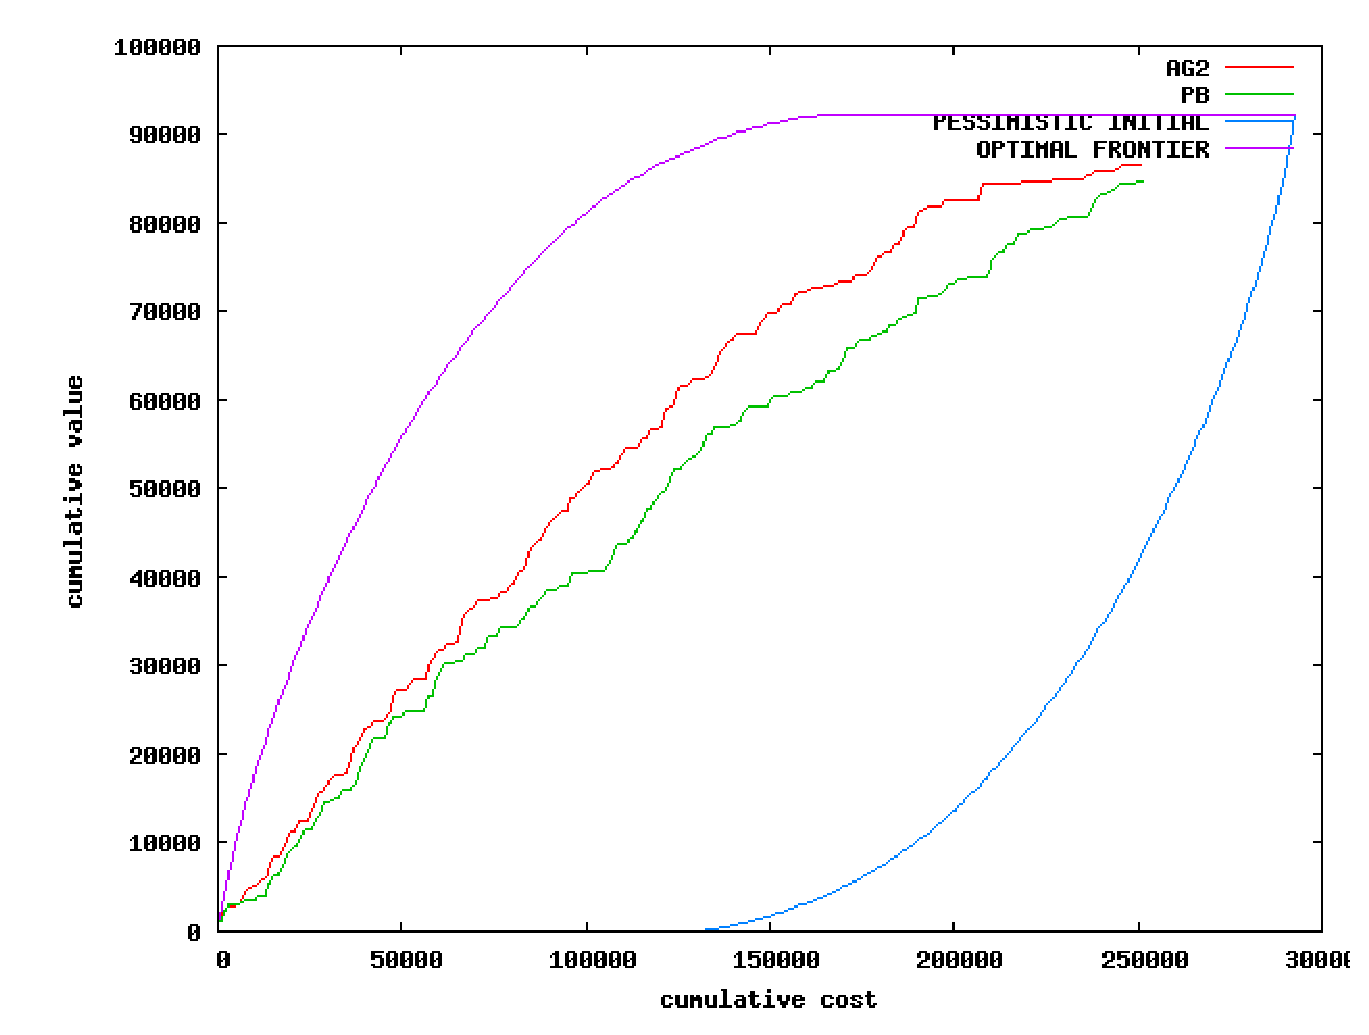
\includegraphics[width=5.35cm]{fakechart.eps}
      \end{minipage}
      \begin{minipage}{7.65cm}
        \begin{equation}\label{eq:score}
          \mathtt{score} = \frac{\int AC - \int PF}{\int OF - \int PF}
        \end{equation}
        By using the area between the OF and PF curve, the project configuration bears no impact on the final score. Thus leaving just the impact of the model inputs and prioritization policy.
      \end{minipage}
    }
\end{kasten}

\begin{kasten}
    \section*{ \hspace{0.1cm} {\color{red} \underline{MODEL INPUTS}}}
    \large{
    POM2 accepted eight input variables.  \textit{Criticality}: affects 
requirements development cost.  \textit{Criticality Modifier}: affects 
the severity of criticality. \textit{Culture}: affects requirements 
reordering and perceived value.  \textit{Initial-known}: sets the
size of the initial requirements set.  \textit{Inter-dependency}: 
frequency of inter-team dependency for requirements.  \textit{Size}: 
size of project (number of requirements).  \textit{Team size}: size of teams 
working on project.  \textit{Dynamism}: how frequently requirements' values 
change.

    }
\end{kasten}

\begin{kasten}
    \section*{ \hspace{0.1cm} {\color{red} \underline{RESULTS}}}
    \tiny
    
\begin{tabular}{@{ } l @{ } r | @{ } r | @{ } r | @{ } r | @{ } r | @{ } r | @{ } r | @{ } r | @{ } r | @{ } r | @{ } r |}
% \multicolumn{2}{c|}{~}&\multicolumn{10}{c}{Note: ranges run $bin_{i} <= value < bin_{i+1}$}\\
%\multicolumn{2}{c|}{~} \\
%\multicolumn{2}{c|}{~} \\
\cline{3-12}
  	&& bin 1 & bin 2 & bin 3 & bin 4 & bin 5 & bin 6 & bin 7 & bin 8 & bin 9 & bin 10 \\
          \cline{2-12}
%          & & & & & & & & & & & \\
	  & criticality
	  & .82
	  & .86
	  & .91
	  & .95
	  & 1.0
	  & 1.04
	  & 1.08
	  & 1.13
	  & 1.17
	  & 1.22\\
	  & criticality modifier
  	  & 2.0
	  & 2.8
	  & 3.6
	  & 4.4
	  & 5.2
	  & 6.0
	  & 6.8
	  & 7.6
	  & 8.4
	  & 9.2\\
	  &culture
	  & 0
	  & 10
	  & 20
	  & 30
	  & 40
	  & 50
	  & 60
	  & 70
	  & 80
	  & 90 \\
	  &initial known
	  & .40
	  & .43
	  & .46
	  & .49
	  & .52
	  & .55
	  & .58
	  & .61
	  & .64
	  & .67\\
	  &inter-dependency
	  & 0
	  & 10
	  & 20
	  & 30
	  & 40
	  & 50
	  & 60
	  & 70
	  & 80
	  & 90\\
	  &size (total personnel)
	  & 3.0
	  & 32.7
	  & 62.4
	  & 92.1
	  & 121.8
	  & 151.5
	  & 181.2
	  & 210.9
	  & 240.6
	  & 270.3\\
policy / dynamism&team size (people per team)
	  & 1.0
	  & 5.1
	  & 9.2
	  & 13.3
	  & 17.4
	  & 21.5
	  & 25.6
	  & 29.7
	  & 33.8
	  & 37.9\\
          

%policy / dynamism \\
\hline
plan-based / very low&criticality&
 &
 &
 &
 &
 &
 &
 &
 &
 &
 \\
$\sigma=\lambda=0$&criticality modifier&
 &
 &
 &
 &
 &
 &
 &
 &
 &
 \\
&culture&
 &
 &
 &
 &
 &
 &
 &
 &
 &
 \\
&initial known     &
 &
 &
 &
 &
 &
 &
 &
 &
\sq{2}{98} &
\sq{4}{96} \\
&inter-dependency     &
 &
 &
 &
 &
 &
 &
\sq{1}{99} &
\sq{1}{99} &
\sq{1}{99} &
 \\
&size     &
\sq{89}{11} &
\sq{2}{98} &
 &
 &
 &
 &
 &
 &
 &
 \\
&team size     &
 &
 &
 &
 &
 &
 &
 &
 &
 &
\sq{1}{99} \\
          \hline
 plan-based / medium&criticality     &
 &
 &
 &
 &
 &
 &
 &
\sq{5}{95} &
\sq{21}{79} &
\sq{52}{48} \\
$\sigma = 0.15, \lambda = 0.0.15$&criticality modifier&
 &
 &
 &
 &
 &
 &
 &
 &
 &
 \\
&culture&
 &
 &
 &
 &
 &
 &
 &
 &
 &
 \\
&initial known&
 &
 &
 &
 &
 &
 &
 &
 &
 &
 \\
&inter-dependency     &
 &
 &
 &
 &
 &
\sq{1}{99} &
\sq{2}{98} &
\sq{6}{94} &
\sq{6}{94} &
\sq{8}{92} \\
&size&
 &
 &
 &
 &
 &
 &
 &
 &
 &
 \\
&team size     &
 &
 &
 &
 &
 &
 &
 &
 &
 &
\sq{1}{99} \\
          \hline
plan-based / very-high &criticality     &
 &
 &
 &
 &
 &
 &
\sq{1}{99} &
\sq{6}{94} &
\sq{22}{78} &
\sq{58}{42} \\
$\sigma=2, \lambda=0.2$&criticality modifier&
 &
 &
 &
 &
 &
 &
 &
 &
 &
 \\
&culture&
 &
 &
 &
 &
 &
 &
 &
 &
 &
 \\
&initial known&
 &
 &
 &
 &
 &
 &
 &
 &
 &
 \\
&inter-dependency     &
 &
 &
 &
 &
 &
\sq{2}{98} &
\sq{3}{97} &
\sq{6}{94} &
\sq{10}{90} &
\sq{11}{89} \\
&size&
 &
 &
 &
 &
 &
 &
 &
 &
 &
 \\
&team size     &
 &
 &
 &
 &
 &
 &
 &
 &
 &
\sq{1}{99} \\
          \hline
agile 2 / very low&criticality&
 &
 &
 &
 &
 &
 &
 &
 &
 &
 \\
$\sigma=\lambda=0$&criticality modifier&
 &
 &
 &
 &
 &
 &
 &
 &
 &
 \\
&culture&
 &
 &
 &
 &
 &
 &
 &
 &
 &
 \\
&initial known     &
 &
 &
 &
 &
 &
 &
\sq{1}{99} &
\sq{4}{96} &
\sq{12}{88} &
\sq{27}{73} \\
&interdependency     &
 &
 &
 &
 &
 &
\sq{1}{99} &
\sq{4}{96} &
\sq{6}{94} &
\sq{5}{95} &
\sq{3}{97} \\
&size     &
\sq{72}{28} &
\sq{1}{99} &
 &
 &
 &
 &
 &
 &
 &
 \\
&team size     &
 &
 &
 &
 &
 &
 &
 &
 &
\sq{1}{99} &
\sq{4}{96} \\
\hline
agile 2 / medium&criticality     &
\sq{1}{99} &
 &
 &
 &
 &
 &
\sq{1}{99} &
\sq{1}{99} &
\sq{1}{99} &
\sq{1}{99} \\
$\sigma=0.15, \lambda=0.015$&criticality modifier     &
 &
 &
 &
 &
 &
 &
\sq{1}{99} &
\sq{1}{99} &
\sq{1}{99} &
\sq{1}{99} \\
&culture     &
 &
 &
 &
 &
 &
\sq{3}{97} &
\sq{10}{90} &
\sq{19}{81} &
\sq{22}{78} &
\sq{29}{71} \\
&initial known     &
 &
 &
 &
 &
\sq{1}{99} &
 &
\sq{2}{98} &
\sq{2}{98} &
\sq{2}{98} &
\sq{2}{98} \\
&interdependency     &
 &
 &
 &
\sq{1}{99} &
\sq{1}{99} &
\sq{1}{99} &
\sq{1}{99} &
 &
\sq{1}{99} &
 \\
&size     &
\sq{97}{3} &
 &
 &
 &
 &
 &
 &
 &
 &
 \\
&team size     &
 &
\sq{17}{83} &
\sq{20}{80} &
\sq{11}{89} &
\sq{6}{94} &
\sq{1}{99} &
 &
 &
 &
 \\
          \hline
agile 2 / very high&criticality     &
\sq{1}{99} &
 &
 &
 &
\sq{1}{99} &
 &
\sq{1}{99} &
\sq{1}{99} &
\sq{1}{99} &
\sq{1}{99} \\
$\sigma=2, \lambda=0.2$&criticality modifier     &
\sq{1}{99} &
\sq{1}{99} &
\sq{1}{99} &
\sq{1}{99} &
\sq{1}{99} &
\sq{1}{99} &
\sq{1}{99} &
 &
\sq{1}{99} &
\sq{1}{99} \\
&culture     &
 &
 &
 &
 &
\sq{1}{99} &
\sq{4}{96} &
\sq{13}{87} &
\sq{17}{83} &
\sq{20}{80} &
\sq{22}{78} \\
&initial known     &
 &
 &
 &
 &
 &
\sq{1}{99} &
\sq{1}{99} &
\sq{1}{99} &
\sq{1}{99} &
\sq{1}{99} \\
&interdependency     &
 &
\sq{1}{99} &
\sq{1}{99} &
\sq{1}{99} &
\sq{1}{99} &
\sq{1}{99} &
\sq{1}{99} &
\sq{1}{99} &
 &
\sq{1}{99} \\
&size     &
\sq{100}{0} &
 &
 &
 &
 &
 &
 &
 &
 &
 \\
&team size     &
 &
\sq{15}{85} &
\sq{18}{82} &
\sq{11}{89} &
\sq{5}{95} &
\sq{2}{98} &
\sq{1}{99} &
 &
 &
\\
\end{tabular}


    \vspace{-.5em}
\end{kasten}
